\documentclass[11pt]{article}

\usepackage[margin=1in]{geometry}
\usepackage{amsmath,amssymb}
\usepackage{graphicx}
\usepackage{booktabs}
\usepackage{array}
\usepackage{longtable}
\usepackage{float}
\usepackage{placeins}
\usepackage{xcolor}
\usepackage[hidelinks]{hyperref}

\graphicspath{{../figures/}}
\setlength{\parskip}{0.5em}
\setlength{\parindent}{0em}

\newcommand{\pauliH}{XX+YY+ZZ}
\newcommand{\exactE}{-29.146168109350}
\newcommand{\hvaE}{-29.037601351802}
\newcommand{\hvaF}{0.982518440088}
\newcommand{\rvbE}{-29.012072100265}
\newcommand{\rvbF}{0.978535993636}

\title{\textbf{Weighted-RVB Initialization and Heisenberg-HVA Refinement\\
for a 19-Site Kagome Antiferromagnetic Heisenberg Benchmark}}
\author{Adel H. Al-Yoorby\\
QIntern 2026 Project qi26\_09\\
Mentor context: Dr. Muhammad Ahsan, QWorld Association, QResearch Department}
\date{July 2026}

\begin{document}
\maketitle

\begin{abstract}
We present a finite-size proof-of-concept for preparing low-energy states of a 19-site Kagome antiferromagnetic Heisenberg model using a signed weighted resonating-valence-bond (RVB) initializer followed by shallow edge-colored Heisenberg Hamiltonian variational ansatz (HVA) layers.  The model is benchmarked by exact sparse diagonalization in the fixed-$S^z$ sector with $n_\downarrow=9$ and Hilbert-space dimension $\binom{19}{9}=92378$.  A static 9-singlet product state gives energy $E=-27.000000$ and fidelity $F=0.014241$ against the exact ground state.  Optimizing signed amplitudes over 54 maximum dimer coverings improves this to $E=\rvbE$ and $F=\rvbF$.  A no-calibration, edge-colored Heisenberg-HVA refinement reaches $E=\hvaE$ and $F=\hvaF$ at depth $p=4$, closing $94.94\%$ of the static-dimer-to-exact energy gap.  Exact calibrated-Hamiltonian reference scans can reach closer finite-size states, with the best reproduced triangle perturbation giving error $3.70\times 10^{-5}$ and fidelity $0.999966$.  The result should therefore be interpreted as a strong no-calibration circuit-refinement baseline and not as a scalable or hardware-ready proof of quantum spin liquid preparation.
\end{abstract}

\section{Introduction}

The spin-$1/2$ Kagome antiferromagnetic Heisenberg model is a canonical frustrated-magnetism benchmark and a central model in the search for quantum spin liquid (QSL) behavior.  The open-boundary 19-site patch studied here is small enough for exact fixed-sector diagonalization yet large enough to expose limitations of purely local dimer product states.

This report studies the following workflow:
\[
\begin{aligned}
&\text{weighted RVB initialization}
\;\longrightarrow\;
\text{edge-colored Heisenberg-HVA refinement}\\
&\hspace{2.4cm}\longrightarrow\;
\text{19-site exact benchmark comparison}.
\end{aligned}
\]
The central question is whether improving the variational state structure can approach the exact 19-site ground state without relying on Hamiltonian calibration.  The answer in this proof-of-concept is cautiously positive: the no-calibration HVA improves energy, fidelity, magnetization, entropy, and bond-correlation diagnostics, but it remains above the best exact calibrated-Hamiltonian reference states.

\section{Provenance and Scope}

The original Ahsan Kagome-VQE material is used as provenance and methodology context, not as code copied into this workflow.  In particular, it provides the source cross-check for the 19-site Kagome connectivity, context for hardware-efficient Qiskit VQE experiments, and the calibrated-Hamiltonian or defect-triangle strategy.  The present proof-of-concept instead develops a separate no-calibration route based on signed weighted-RVB initialization and shallow edge-colored Heisenberg-HVA refinement.

\begin{table}[H]
\centering
\caption{Role of each component in the final project narrative.}
\label{tab:component_roles}
\begin{tabular}{p{0.33\textwidth}p{0.57\textwidth}}
\toprule
Component & Role \\
\midrule
External Ahsan Kagome-VQE material & Original calibrated-Hamiltonian/VQE provenance and future hardware-method context. \\
19-site bond list & Confirmed against the Ahsan notebook and used as the active benchmark graph. \\
Weighted RVB & Main physics initializer and dominant improvement over static dimers. \\
Heisenberg-HVA & No-calibration circuit-refinement path. \\
Calibration scans & Exact-state reference comparison, not the main no-calibration claim. \\
ODR / IBM Runtime ideas & Future hardware and noise-mitigation extension. \\
\bottomrule
\end{tabular}
\end{table}

When discussing the original calibrated-Hamiltonian direction, we use cautious language: defect or triangle couplings are increased above the uniform value, with reported calibrated values depending on the patch, Hamiltonian convention, defect set, and scan.  This report states precise calibration values only for scans reproduced in the current repository.

\section{Model and Benchmark}

The active Hamiltonian uses the unscaled Pauli convention
\begin{equation}
H = \sum_{\langle i,j\rangle \in E}
\left(X_iX_j + Y_iY_j + Z_iZ_j\right),
\label{eq:hamiltonian}
\end{equation}
where $E$ is the 30-bond 19-site Kagome patch.  Physical spin energies are one quarter of Eq.~\eqref{eq:hamiltonian}:
\[
H_{\rm phys} = \sum_{\langle i,j\rangle} \mathbf{S}_i\cdot\mathbf{S}_j
= \frac{1}{4}H.
\]

The exact reference is the lowest eigenstate in the $n_\downarrow=9$ fixed-$S^z$ sector:
\[
E_0 = \exactE.
\]
All reported fidelities use
\begin{equation}
F(\psi)=|\langle \psi_{\rm exact}|\psi\rangle|^2.
\end{equation}

\subsection{Edge Coloring}

The 30 bonds are partitioned into four disjoint matchings.  Within each matching, all two-qubit Heisenberg gates commute on disjoint qubits and may be applied in parallel.  This converts a bond-dependent layer with 30 parameters into an edge-colored HVA layer with only four parameters.

\begin{table}[H]
\centering
\caption{Four-color edge grouping used by the HVA.  Bonds inside each group are disjoint.}
\label{tab:edge_coloring}
\resizebox{\textwidth}{!}{%
\begin{tabular}{cl}
\toprule
Group & Bonds \\
\midrule
0 & $(1,2),(4,6),(8,10),(11,12),(14,16),(17,18)$ \\
1 & $(0,1),(2,4),(6,8),(10,11),(12,14),(16,17)$ \\
2 & $(2,3),(4,5),(6,7),(8,9),(10,12),(13,14),(15,16),(1,11),(0,17)$ \\
3 & $(3,4),(5,6),(7,8),(9,10),(12,13),(14,15),(16,18),(2,11),(1,17)$ \\
\bottomrule
\end{tabular}}
\end{table}

\section{Variational States}

\subsection{Static Dimer Baseline}

The simplest control state is a product of nine singlets over a greedy maximum matching, leaving one unpaired spin in the 19-site odd patch:
\[
|s_{ij}\rangle = \frac{|0_i1_j\rangle-|1_i0_j\rangle}{\sqrt{2}}.
\]
This state is hardware transparent but too rigid: it reaches $E=-27.000000$ and has fidelity only $F=0.014241$.

\subsection{Signed Weighted-RVB Initializer}

The RVB ansatz is a linear combination of all 54 deterministic maximum dimer coverings:
\begin{equation}
|\psi_{\rm RVB}(c)\rangle =
\sum_{\alpha=1}^{54} c_\alpha |D_\alpha\rangle .
\end{equation}
The coefficients are obtained classically by solving the generalized eigenproblem
\begin{equation}
H_{\alpha\beta}c_\beta = E\,S_{\alpha\beta}c_\beta,
\quad
H_{\alpha\beta}=\langle D_\alpha|H|D_\beta\rangle,
\quad
S_{\alpha\beta}=\langle D_\alpha|D_\beta\rangle.
\end{equation}
The equal positive RVB superposition is a poor approximation, but optimized signs and amplitudes are essential: the weighted RVB state reaches $E=\rvbE$ and $F=\rvbF$.

\subsection{Heisenberg-HVA Refinement}

Starting from the weighted-RVB initializer, the edge-colored HVA applies Heisenberg interactions with one shared parameter per color and layer:
\begin{equation}
|\psi_p(\theta)\rangle =
\left[
\prod_{\ell=1}^{p}
\prod_{c=0}^{3}
\prod_{(i,j)\in E_c}
\exp\left[-i\theta_{\ell,c}\left(X_iX_j+Y_iY_j+Z_iZ_j\right)\right]
\right]
|\psi_{\rm RVB}\rangle .
\label{eq:hva}
\end{equation}
Thus the depth-$p$ edge-colored HVA has $4p$ parameters.  The reported serious run uses a Nelder-Mead optimization with $p=0,1,2,3,4$ cached in the current release artifacts.

\section{Diagnostics}

The analysis tracks more than energy.  For each state, the repository computes fidelity, selected bipartite entropies, maximum site magnetization, bond correlations, and bond-correlation errors relative to the exact state.

For a bond $(i,j)$, the plotted correlation is
\begin{equation}
C_{ij}=\langle X_iX_j+Y_iY_j+Z_iZ_j\rangle.
\end{equation}
A perfect singlet has $C_{ij}=-3$.  The antiferromagnetic bond participation diagnostic is
\begin{equation}
p_{ij} = \frac{\max(0,-C_{ij})}{\sum_{(k,l)}\max(0,-C_{kl})},
\quad
P_{\rm AF} = \frac{1}{\sum_{ij}p_{ij}^2}.
\end{equation}
Large $P_{\rm AF}$ indicates more distributed antiferromagnetic correlation weight.  The figures use a deterministic graph layout for visualization, not a physical Kagome embedding.

\section{Results}

\begin{figure}[H]
\centering
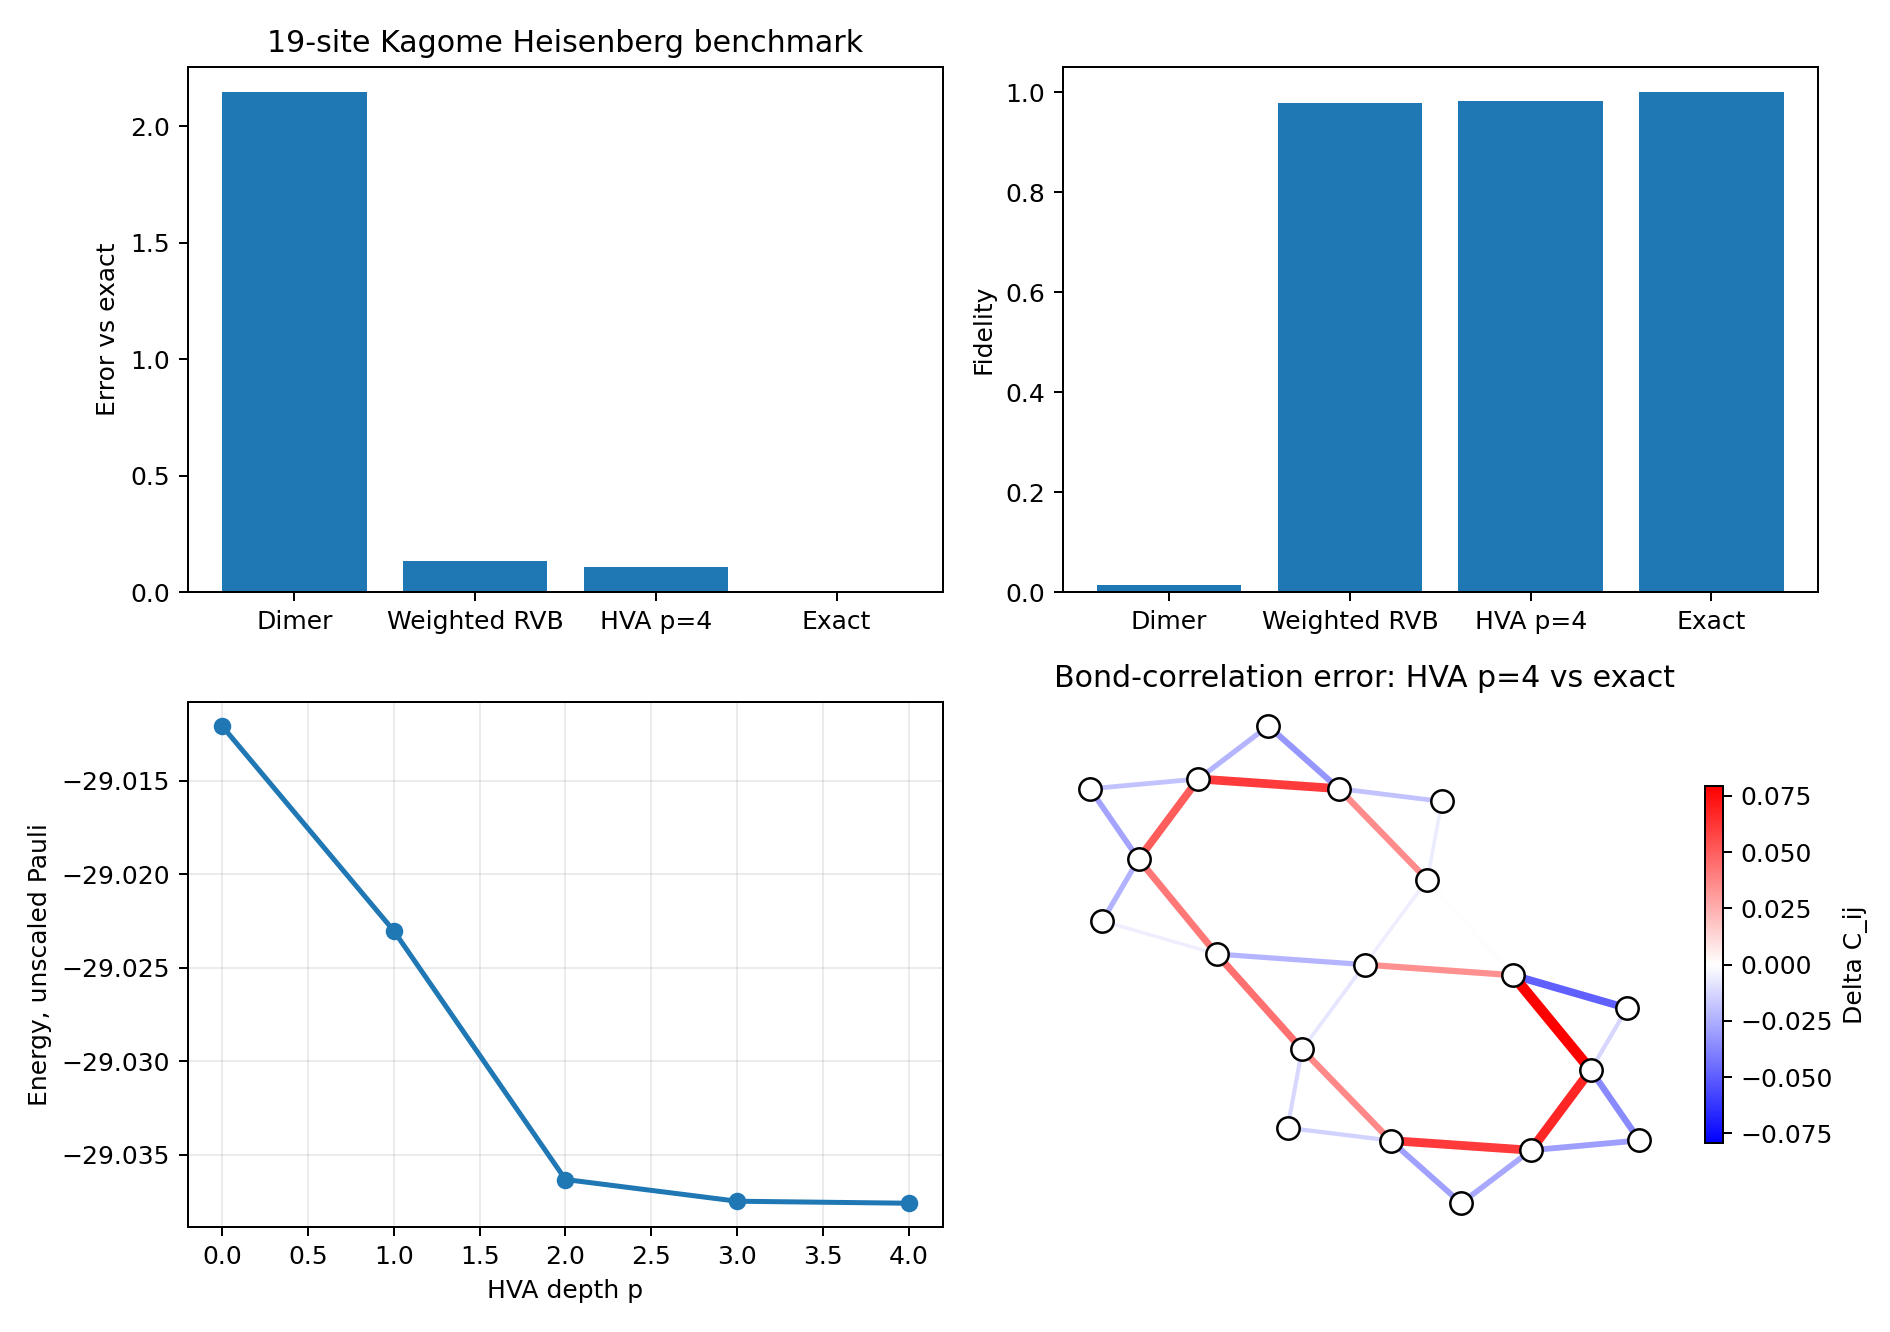
\includegraphics[width=\textwidth]{one_page_summary.png}
\caption{One-page summary of the 19-site benchmark.  The weighted-RVB initializer dramatically improves on the static dimer product state, and Heisenberg-HVA refinement gives a smaller but consistent no-calibration improvement through $p=4$.}
\label{fig:one_page}
\end{figure}

\begin{table}[H]
\centering
\caption{Main exact-benchmark results in the unscaled Pauli convention.  Error is relative to $E_0=\exactE$.}
\label{tab:main_results}
\resizebox{\textwidth}{!}{%
\begin{tabular}{lrrrrrrr}
\toprule
State & Depth & Energy & Error & Fidelity & Gap closed & Entropy & Max mag. \\
\midrule
Static dimer & 0 & -27.00000000 & 2.14616811 & 0.014241 & 0.00\% & 1.000000 & 0.500000 \\
Equal RVB-54 & 0 & -26.39781307 & 2.74835504 & 0.004371 & -28.06\% & 3.366154 & 0.129849 \\
Weighted RVB-54 & 0 & -29.01207210 & 0.13409601 & 0.978536 & 93.75\% & 3.129502 & 0.107755 \\
Weighted RVB + HVA & 1 & -29.02302627 & 0.12314184 & 0.979995 & 94.26\% & 3.129583 & 0.107528 \\
Weighted RVB + HVA & 2 & -29.03633182 & 0.10983629 & 0.982446 & 94.88\% & 3.140691 & 0.104773 \\
Weighted RVB + HVA & 3 & -29.03749397 & 0.10867414 & 0.982442 & 94.94\% & 3.141921 & 0.104388 \\
Weighted RVB + HVA & 4 & -29.03760135 & 0.10856676 & 0.982518 & 94.94\% & 3.155489 & 0.104055 \\
Exact & -- & -29.14616811 & 0.00000000 & 1.000000 & 100.00\% & 3.212669 & 0.094007 \\
\bottomrule
\end{tabular}}
\end{table}

\subsection{Depth Dependence}

\begin{figure}[H]
\centering
\begin{minipage}{0.48\textwidth}
\centering
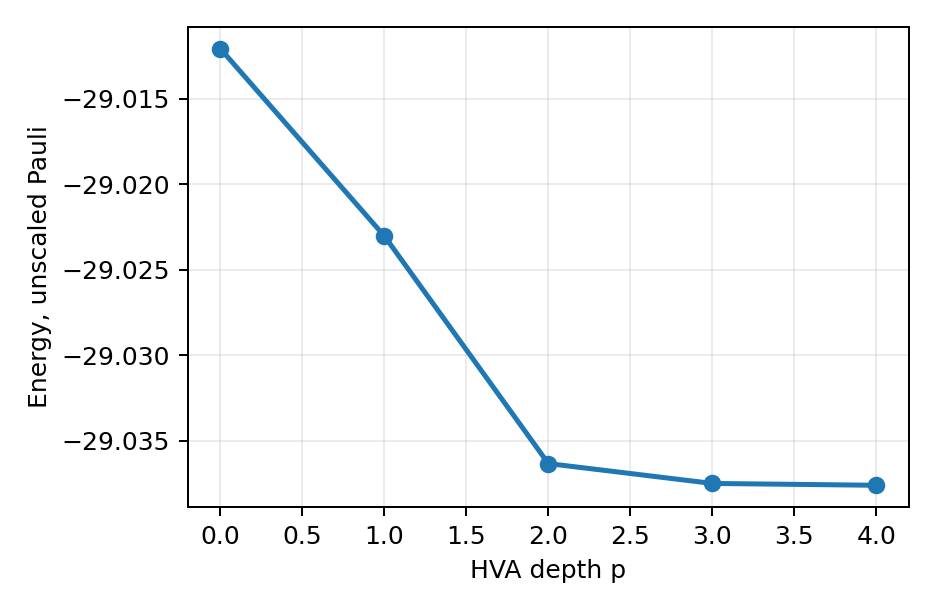
\includegraphics[width=\linewidth]{energy_vs_hva_depth.png}
\end{minipage}
\begin{minipage}{0.48\textwidth}
\centering
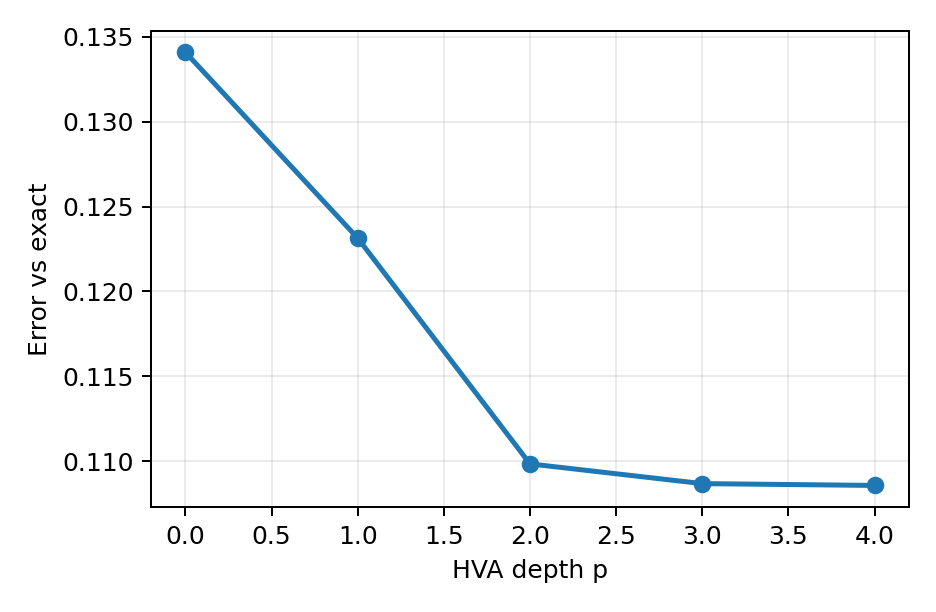
\includegraphics[width=\linewidth]{error_vs_hva_depth.png}
\end{minipage}
\begin{minipage}{0.48\textwidth}
\centering
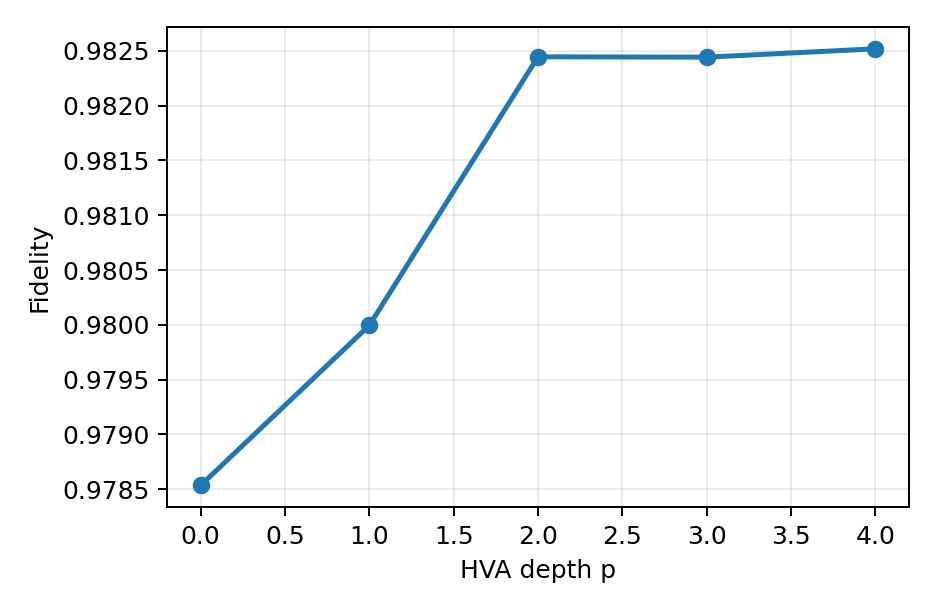
\includegraphics[width=\linewidth]{fidelity_vs_hva_depth.png}
\end{minipage}
\begin{minipage}{0.48\textwidth}
\centering
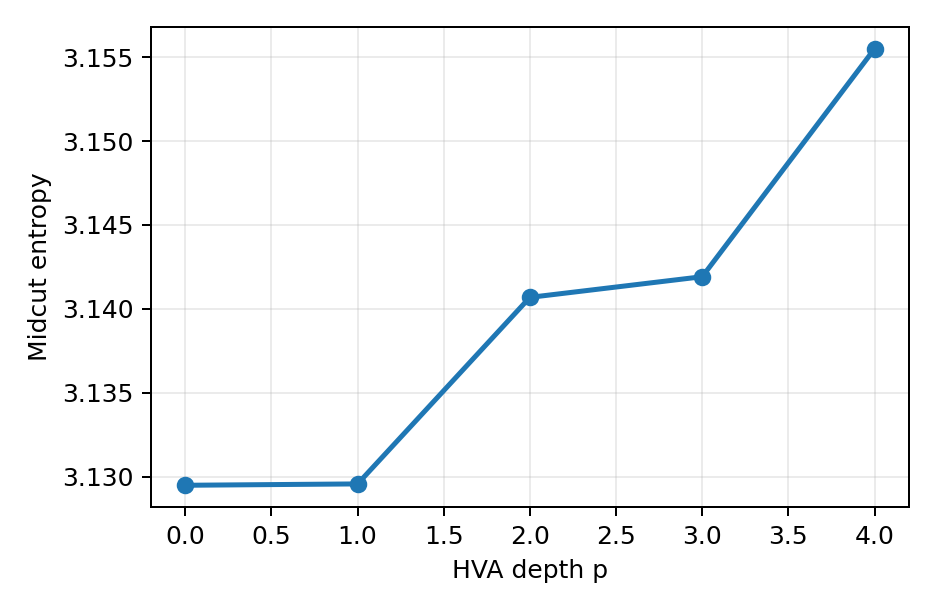
\includegraphics[width=\linewidth]{entropy_vs_hva_depth.png}
\end{minipage}
\caption{Depth dependence of energy, error, fidelity, and entropy.  The largest improvement comes from weighted-RVB initialization; HVA layers provide a smaller additional circuit-compatible refinement.}
\label{fig:depth_energy}
\end{figure}

\begin{figure}[H]
\centering
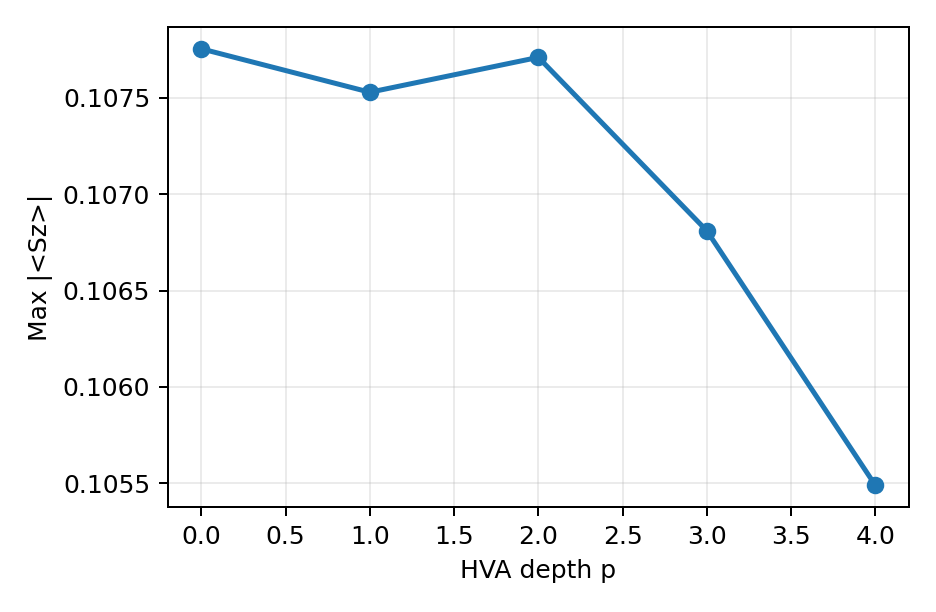
\includegraphics[width=0.62\textwidth]{magnetization_vs_hva_depth.png}
\caption{Maximum site magnetization versus HVA depth.  The weighted RVB and HVA-refined states remain much closer to the low-magnetization exact state than the static dimer baseline.}
\label{fig:magnetization}
\end{figure}

\subsection{Bond-Correlation Structure}

\begin{figure}[H]
\centering
\begin{minipage}{0.48\textwidth}
\centering
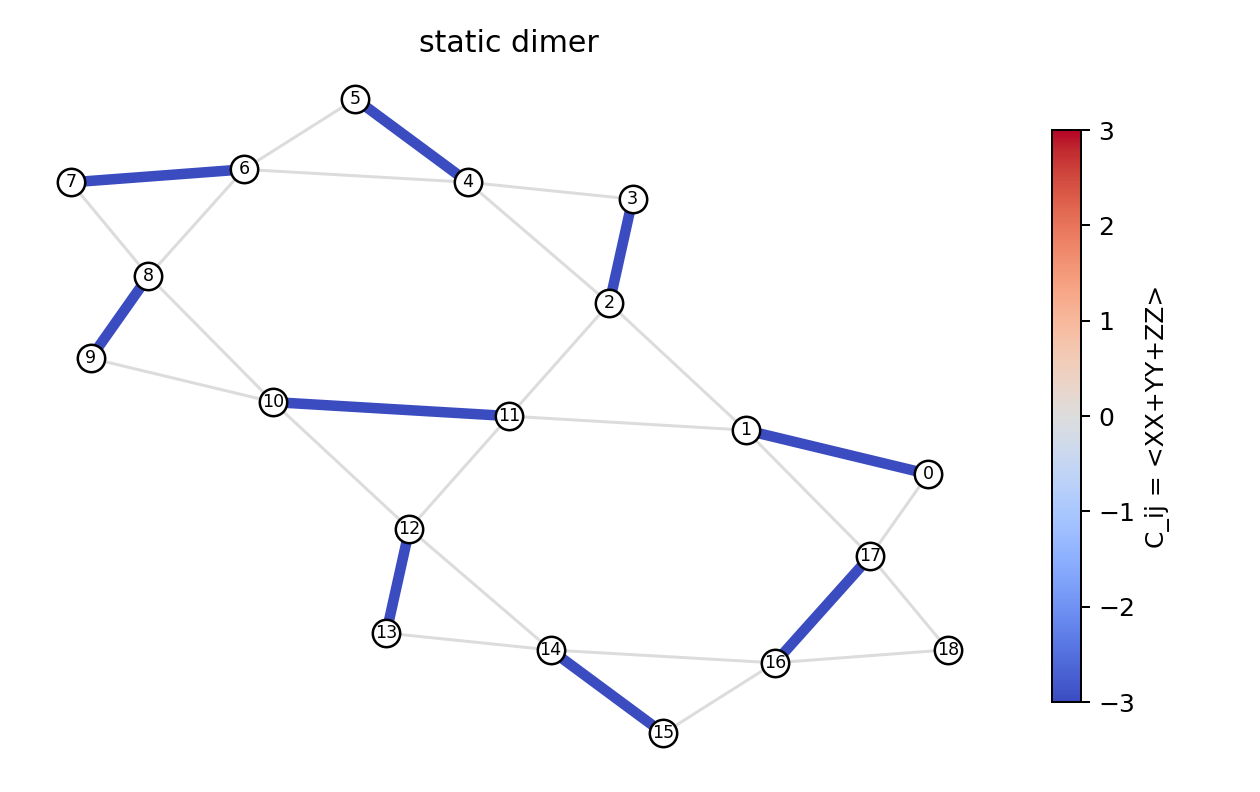
\includegraphics[width=\linewidth]{bond_map_static_dimer.png}
\end{minipage}
\begin{minipage}{0.48\textwidth}
\centering
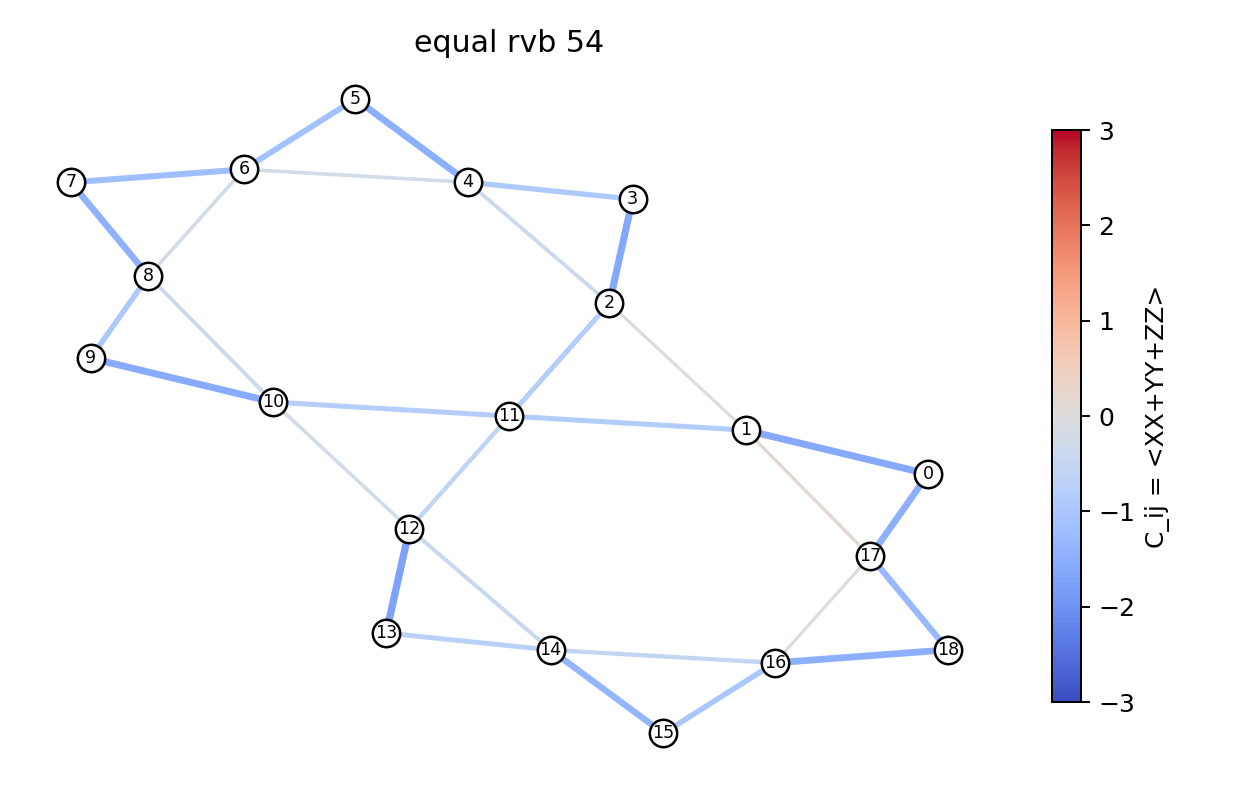
\includegraphics[width=\linewidth]{bond_map_equal_rvb.png}
\end{minipage}
\begin{minipage}{0.48\textwidth}
\centering
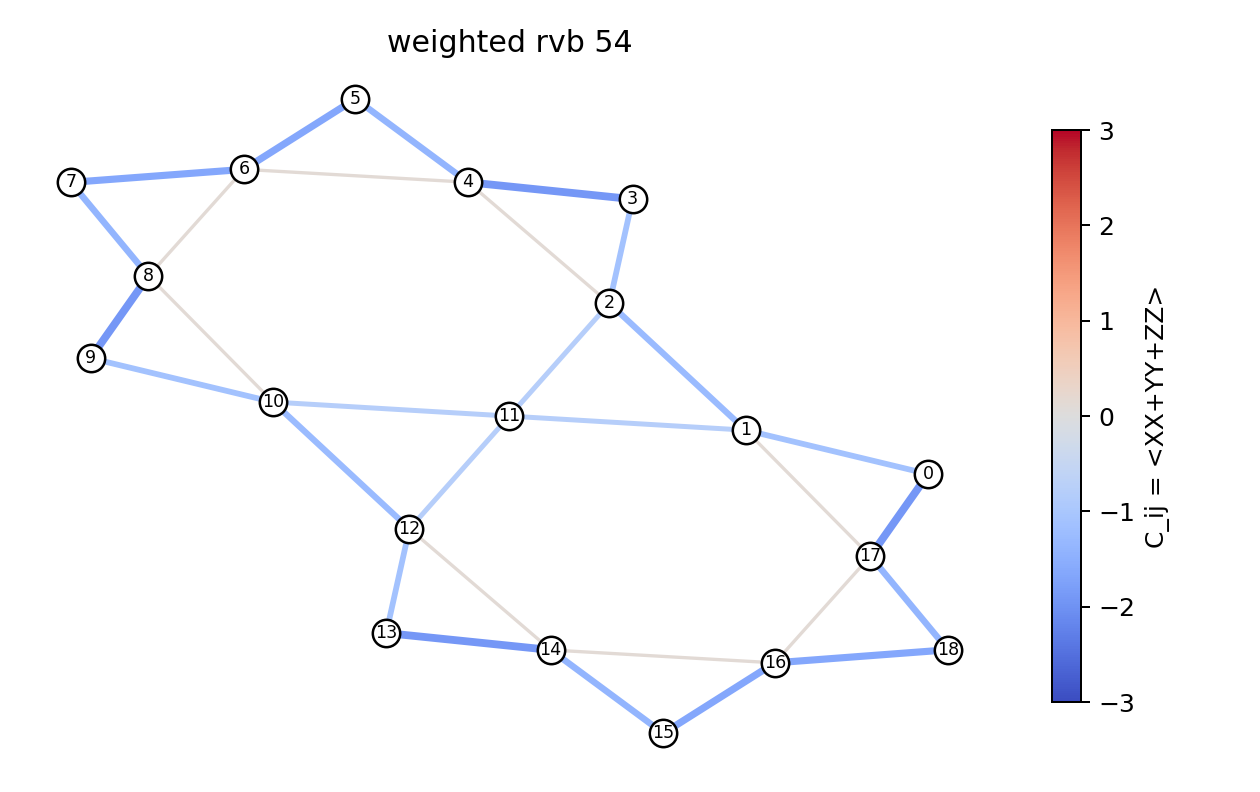
\includegraphics[width=\linewidth]{bond_map_weighted_rvb.png}
\end{minipage}
\begin{minipage}{0.48\textwidth}
\centering
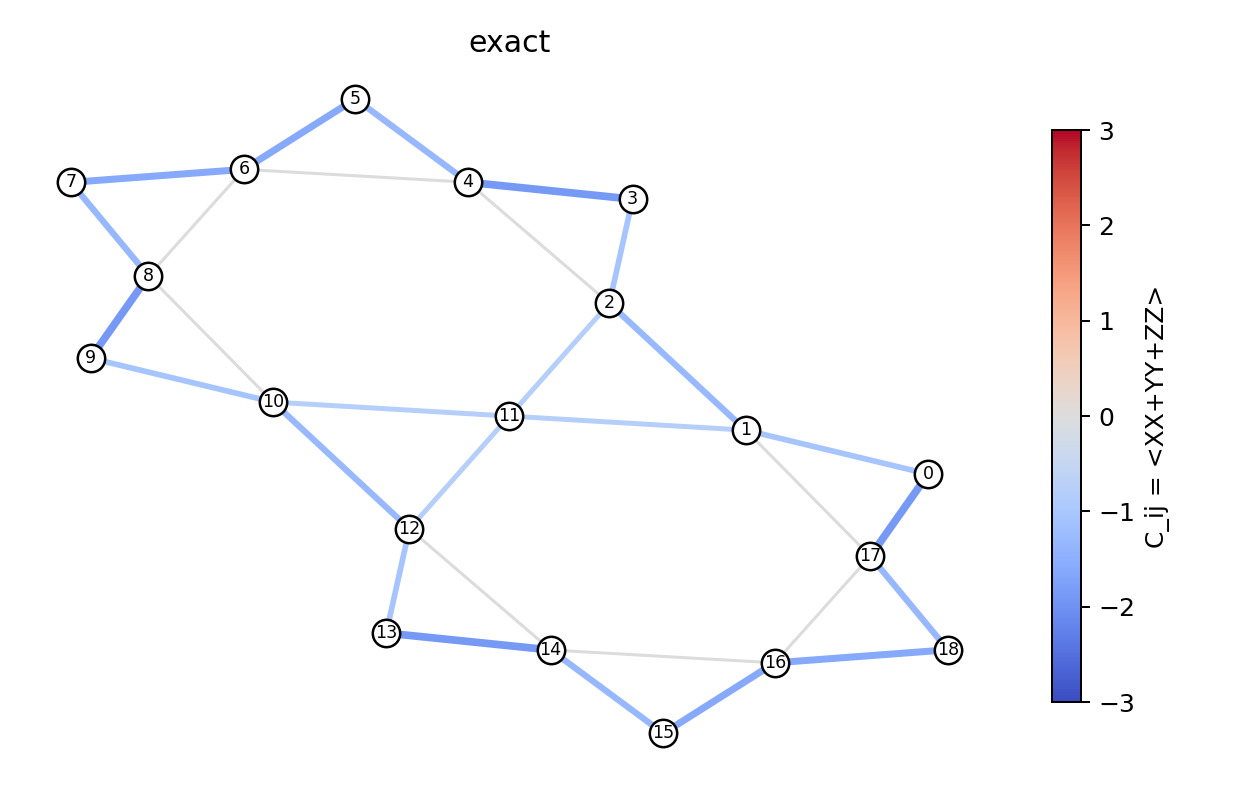
\includegraphics[width=\linewidth]{bond_map_exact.png}
\end{minipage}
\caption{Bond correlations for the static dimer baseline, equal RVB, weighted RVB, and exact state.  The weighted-RVB state captures the exact correlation pattern much better than either the static product state or equal positive RVB.}
\label{fig:bond_core}
\end{figure}

\begin{figure}[H]
\centering
\begin{minipage}{0.48\textwidth}
\centering
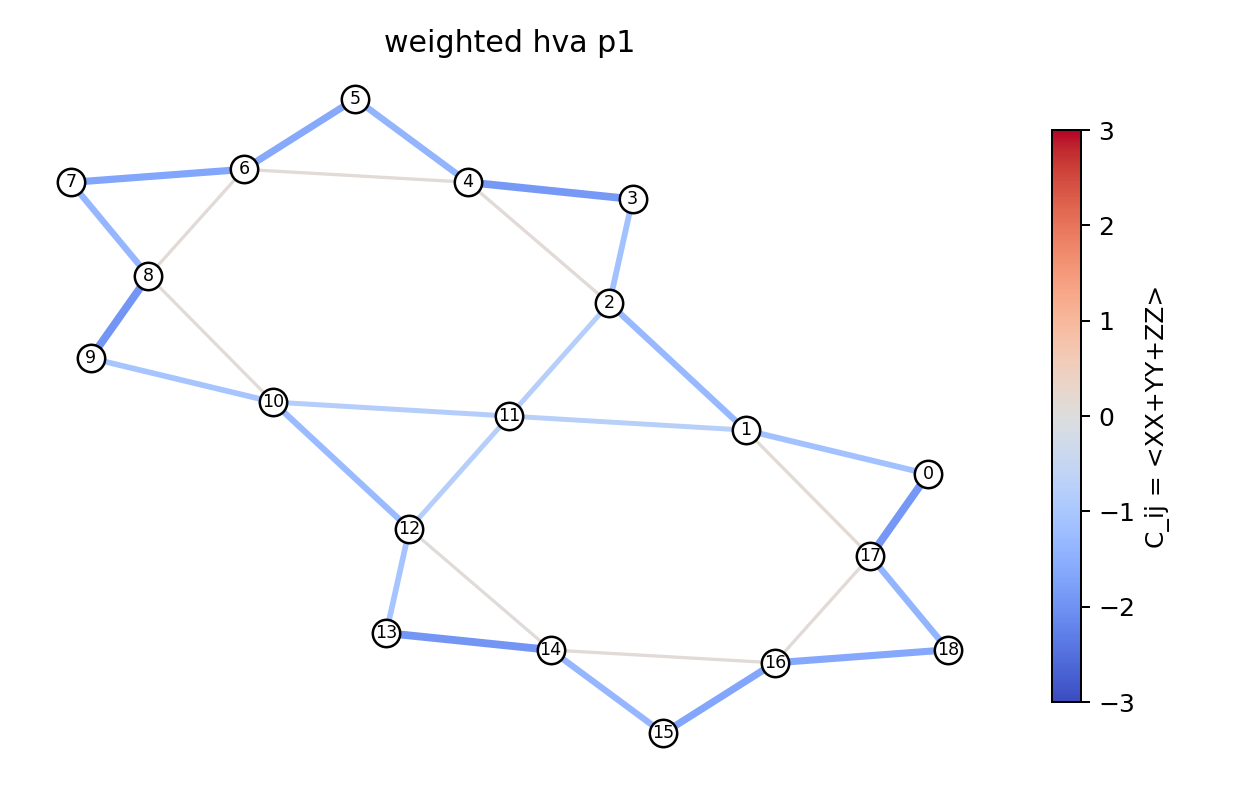
\includegraphics[width=\linewidth]{bond_map_weighted_hva_p1.png}
\end{minipage}
\begin{minipage}{0.48\textwidth}
\centering
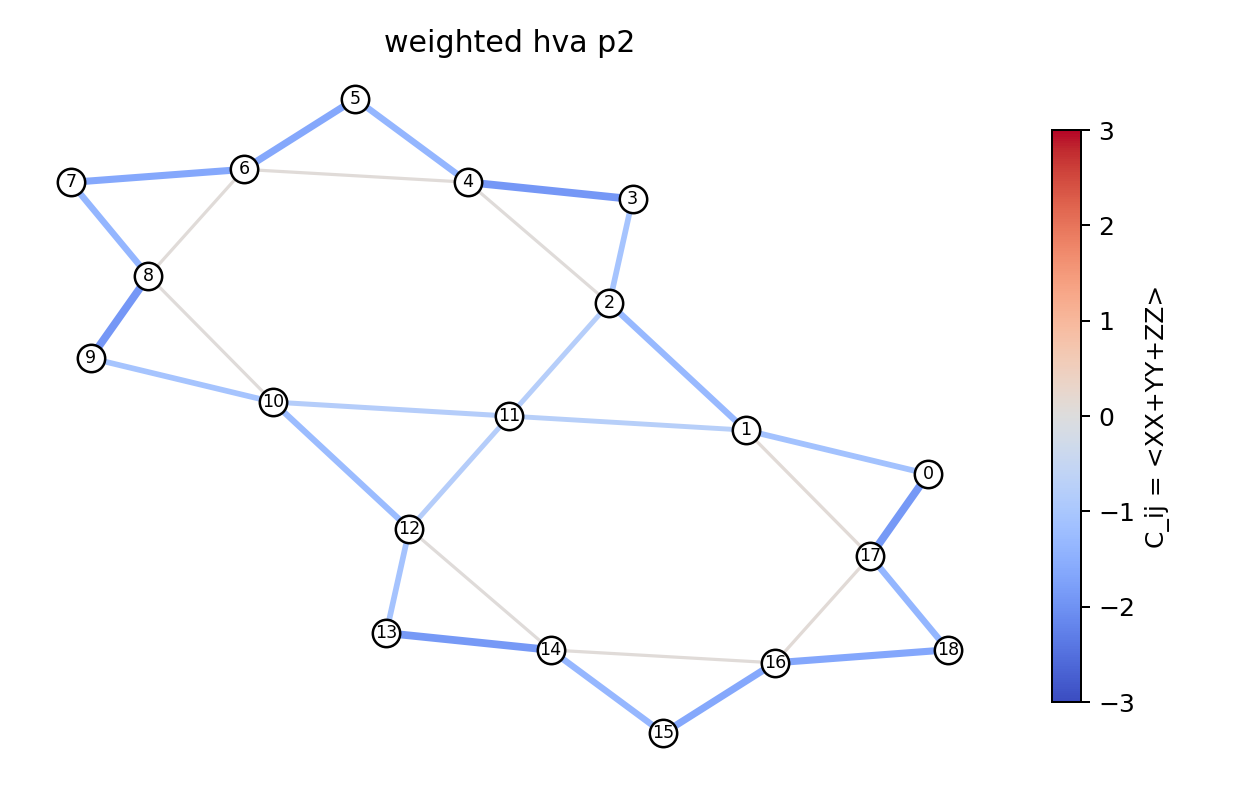
\includegraphics[width=\linewidth]{bond_map_weighted_hva_p2.png}
\end{minipage}
\begin{minipage}{0.48\textwidth}
\centering
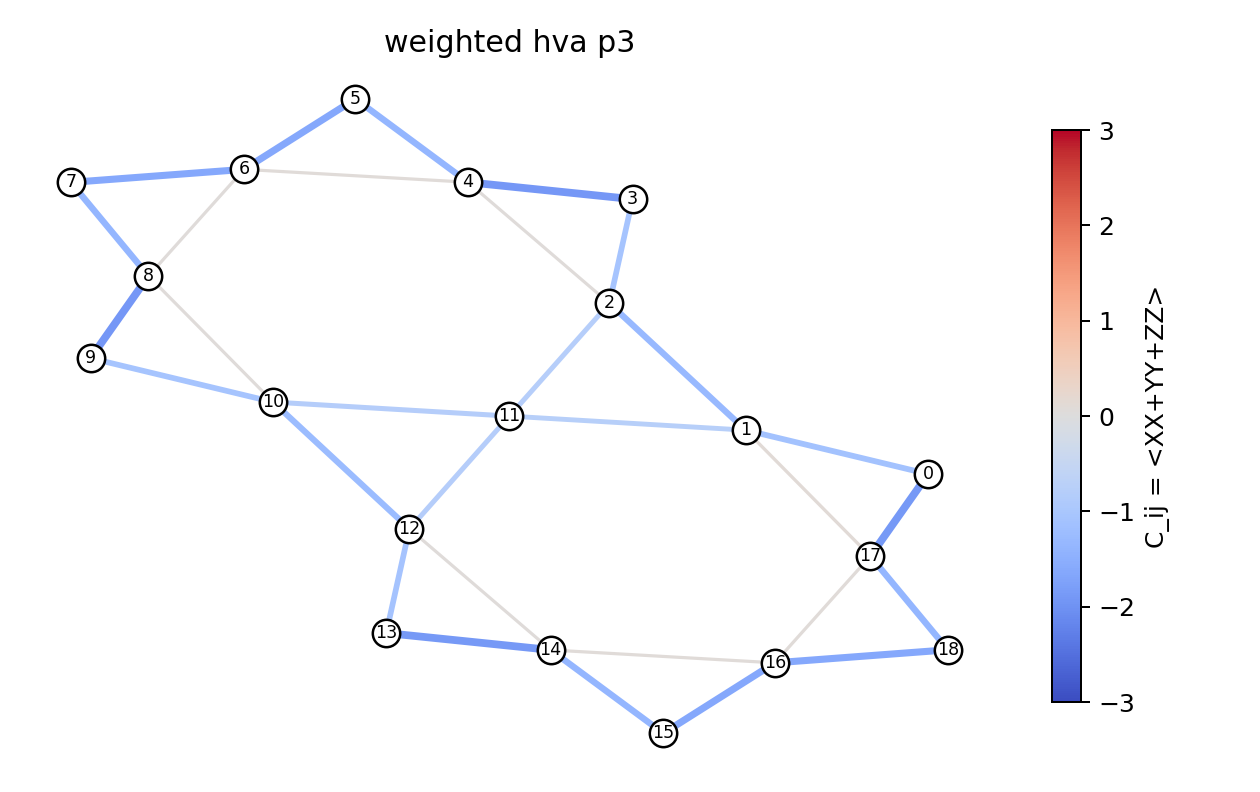
\includegraphics[width=\linewidth]{bond_map_weighted_hva_p3.png}
\end{minipage}
\begin{minipage}{0.48\textwidth}
\centering
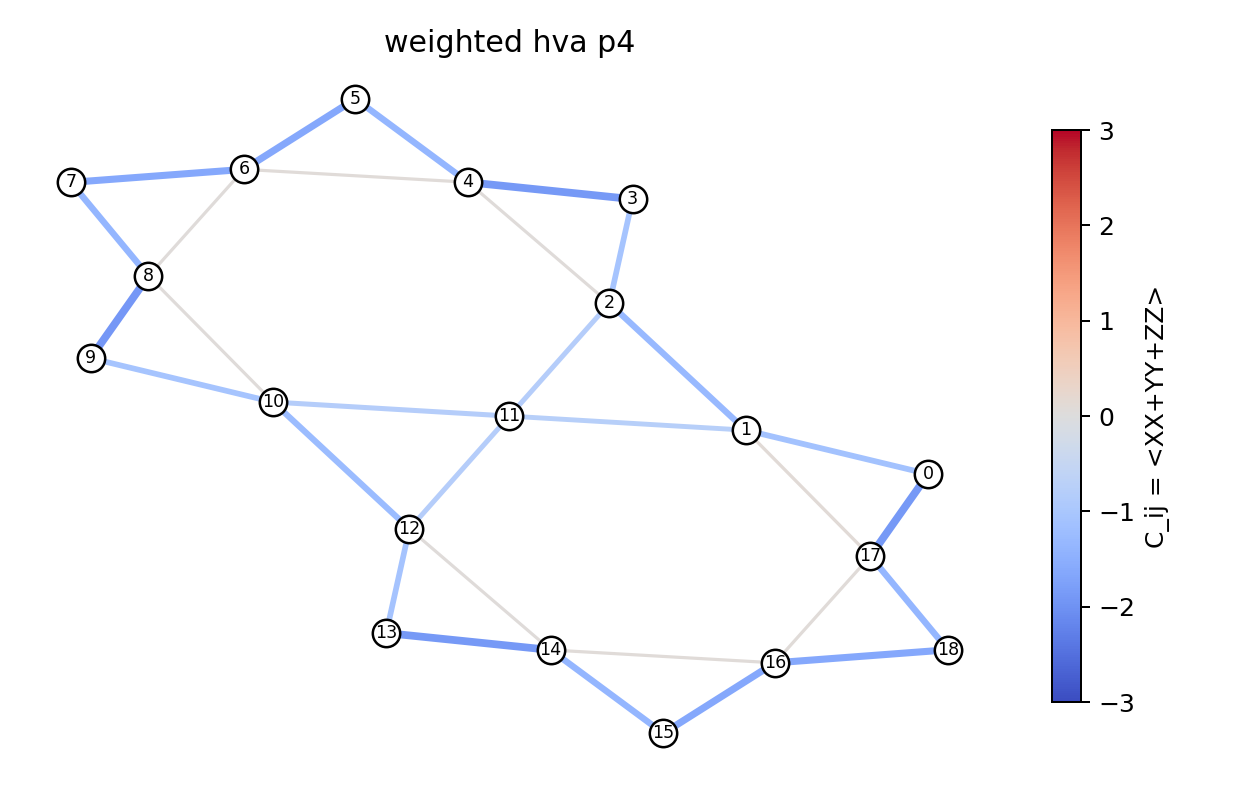
\includegraphics[width=\linewidth]{bond_map_weighted_hva_p4.png}
\end{minipage}
\caption{Bond-correlation maps after HVA refinement at $p=1,2,3,4$.  Refinement is incremental but consistently preserves the distributed antiferromagnetic structure of the weighted-RVB initializer.}
\label{fig:bond_hva}
\end{figure}

\begin{figure}[H]
\centering
\begin{minipage}{0.48\textwidth}
\centering
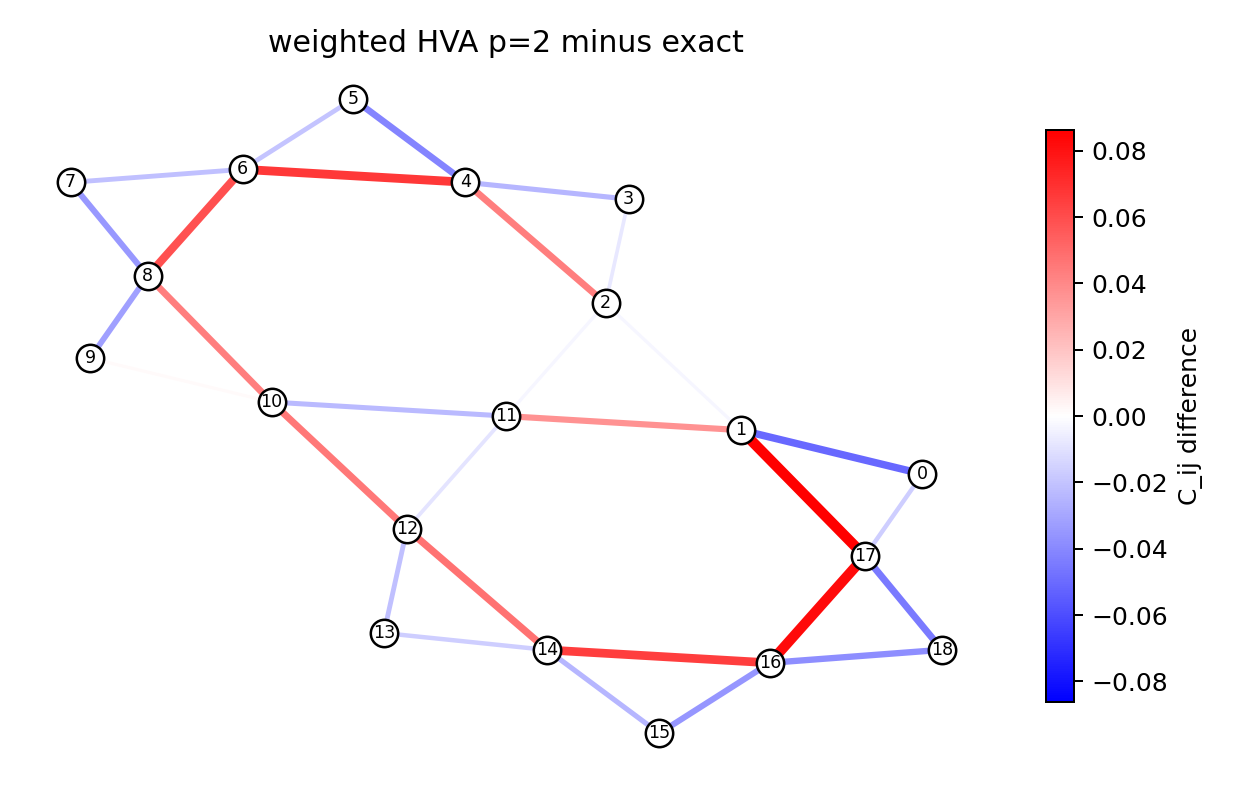
\includegraphics[width=\linewidth]{bond_map_error_p2_vs_exact.png}
\end{minipage}
\begin{minipage}{0.48\textwidth}
\centering
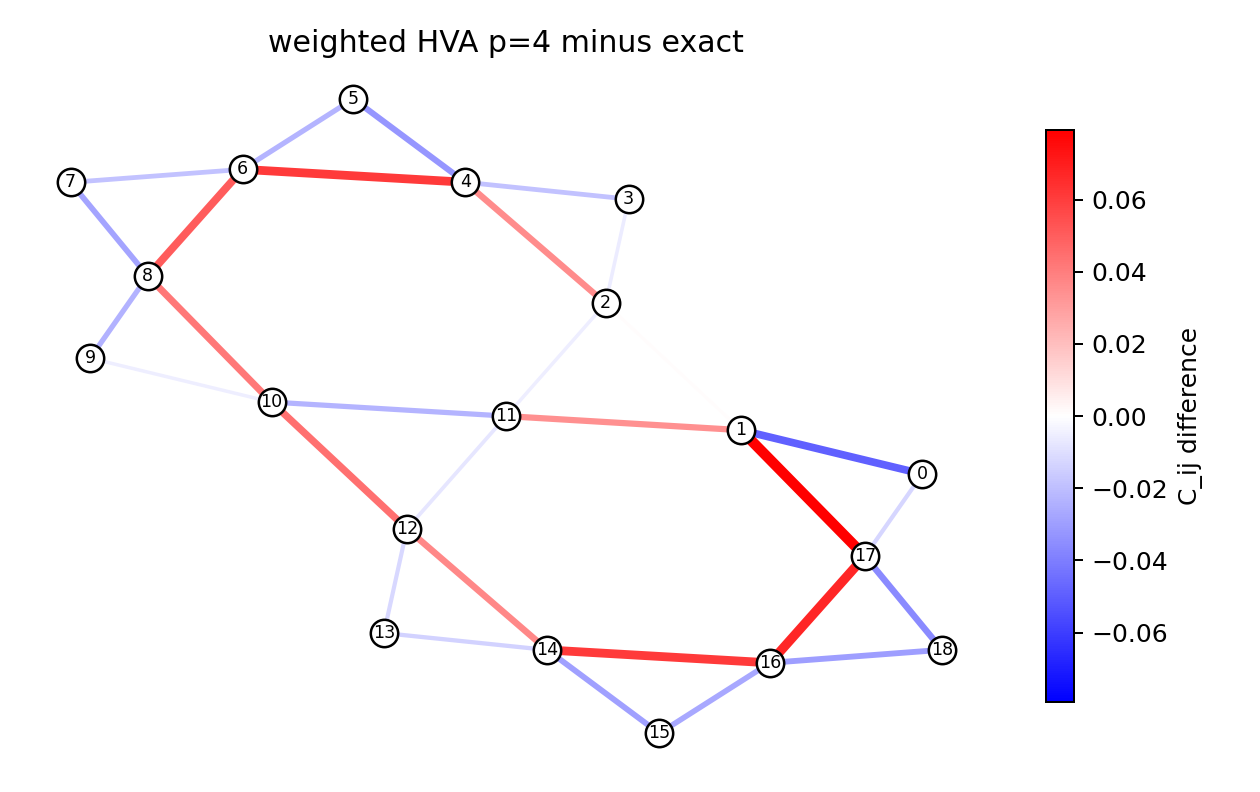
\includegraphics[width=\linewidth]{bond_map_error_best_hva_vs_exact.png}
\end{minipage}
\caption{Bond-correlation error maps relative to the exact state.  Left: earlier $p=2$ HVA reference.  Right: best current no-calibration HVA, $p=4$.}
\label{fig:bond_error}
\end{figure}

\subsection{Calibration Reference Comparison}

The no-calibration HVA result should be compared honestly against exact calibrated-Hamiltonian reference scans.  In those scans, the ground state of a modified Hamiltonian is obtained exactly and then evaluated against the original target Hamiltonian.  This is a reference-state diagnostic, not a direct hardware-preparable circuit comparison.

\begin{table}[H]
\centering
\caption{No-calibration HVA compared with reproduced calibrated-Hamiltonian exact references.}
\label{tab:calibration}
\begin{tabular}{lrr}
\toprule
Method & Energy error & Fidelity \\
\midrule
Weighted RVB + HVA $p=4$ & 0.108567 & 0.982518 \\
Calibrated group color1, $J'=1.02$ & 0.003945 & 0.994967 \\
Calibrated bond 14--16, $J'=1.02$ & 0.000510 & 0.999626 \\
Calibrated triangle 6--7--8, $J'=1.02$ & 0.000037 & 0.999966 \\
\bottomrule
\end{tabular}
\end{table}

\begin{figure}[H]
\centering
\begin{minipage}{0.48\textwidth}
\centering

\includegraphics[width=\linewidth]{calibration_energy_vs_fidelity.png}
\end{minipage}
\begin{minipage}{0.48\textwidth}
\centering

\includegraphics[width=\linewidth]{calibration_energy_vs_fidelity_zoom.png}
\end{minipage}
\caption{Calibration scan landscape.  The exact calibrated-Hamiltonian references can sit much closer to the target exact state than the current no-calibration HVA baseline.}
\label{fig:calibration}
\end{figure}

\section{Discussion}

The main scientific observation is that the signs and amplitudes of dimer coverings matter strongly.  Equal RVB over the 54 maximum coverings performs worse than a static dimer product, while signed weighted RVB jumps to high fidelity.  This indicates that the relevant finite-size spin-liquid-like structure is not merely a uniform superposition of local singlet coverings; it requires phase and amplitude structure in the dimer-covering manifold.

The HVA contribution is more modest but important.  The $p=4$ edge-colored Heisenberg-HVA result improves the weighted-RVB energy from $-29.01207210$ to $-29.03760135$ and fidelity from $0.978536$ to $0.982518$ without Hamiltonian calibration.  This is not enough to match the exact calibrated-Hamiltonian references, but it demonstrates that a physically structured two-qubit Heisenberg ansatz can refine a high-quality RVB state in the direction of the exact finite-size ground state.

The result is also useful because it separates two routes that were previously entangled in the project narrative:
\[
\text{state-structure improvement}
\quad\text{versus}\quad
\text{Hamiltonian calibration}.
\]
The calibrated-Hamiltonian route remains powerful as an exact-state reference.  The no-calibration HVA route is the cleaner circuit-refinement proof-of-concept.

\section{Limitations}

\begin{itemize}
\item The result is finite-size only and uses a 19-site open-boundary patch.
\item The exact benchmark is in the fixed $S^z=1/2$ sector.
\item The weighted-RVB initializer is obtained by a classical generalized eigenproblem and is not yet a hardware-preparable state-preparation circuit.
\item The Heisenberg-HVA improvement is real but modest through $p=4$.
\item The no-calibration HVA does not outperform the best exact calibrated-Hamiltonian reference scan in energy or fidelity.
\item No repeated-optimizer statistical robustness campaign is included in this frozen package.
\item No noise model, Qiskit Runtime execution, or hardware experiment is included.
\item No scalable QSL preparation claim is made.
\end{itemize}

\section{Reproducibility}

The main repository artifacts are:
\begin{itemize}
\item \texttt{data/19site\_bonds.csv}: active 19-site bond list and edge coloring.
\item \texttt{results/final\_result\_table.csv}: main result table.
\item \texttt{results/no\_calibration\_vs\_best\_calibration.csv}: compact comparison of the best HVA and best calibration reference.
\item \texttt{results/19site\_heisenberg\_hva\_fast\_weighted\_p4\_neldermead\_*.csv}: current best serious no-calibration HVA output.
\item \texttt{figures/}: all plots included in this report.
\end{itemize}

The default quick reproduction path is:
\begin{verbatim}
.\run_all.ps1
\end{verbatim}
or, on Unix-like systems,
\begin{verbatim}
bash run_all.sh
\end{verbatim}
The serious $p=4$ optimizer path can take hours and is cached in the current release artifacts.

\section{Conclusion}

This proof-of-concept establishes a clean finite-size baseline for a 19-site Kagome Heisenberg patch.  A signed weighted-RVB initializer captures most of the exact-state structure, and a shallow edge-colored Heisenberg-HVA gives additional no-calibration circuit-compatible refinement.  The best current no-calibration HVA result reaches
\[
E=\hvaE,\quad F=\hvaF,
\]
with an energy error of $0.10856676$ relative to the exact benchmark.  The result is strong enough to motivate deeper or more expressive Heisenberg-level ansatz work, but the present evidence remains finite-size and does not claim scalable hardware QSL preparation.

\begin{thebibliography}{9}

\bibitem{yan2011}
S. Yan, D. A. Huse, and S. R. White,
``Spin-liquid ground state of the $S=1/2$ kagome Heisenberg antiferromagnet,''
\emph{Science} \textbf{332}, 1173--1176 (2011).

\bibitem{peruzzo2014}
A. Peruzzo \emph{et al.},
``A variational eigenvalue solver on a photonic quantum processor,''
\emph{Nature Communications} \textbf{5}, 4213 (2014).

\bibitem{kandala2017}
A. Kandala, A. Mezzacapo, K. Temme, M. Takita, M. Brink, J. M. Chow, and J. M. Gambetta,
``Hardware-efficient variational quantum eigensolver for small molecules and quantum magnets,''
\emph{Nature} \textbf{549}, 242--246 (2017).

\bibitem{farhi2014}
E. Farhi, J. Goldstone, and S. Gutmann,
``A quantum approximate optimization algorithm,''
arXiv:1411.4028 (2014).

\bibitem{qiskit}
Qiskit Community,
``Qiskit: An open-source framework for quantum computing,''
Zenodo, doi:10.5281/zenodo.2562110 (2017).

\end{thebibliography}

\end{document}
